
\chapter{Teste\label{chap:Teste}}

\lhead{\thechapter - Teste} 

Todo projeto de engenharia passa por uma etapa de testes. Neste cap�tulo
apresentamos alguns testes do software desenvolvido. Estes testes
devem dar resposta aos diagramas de caso de uso inicialmente apresentados
(diagramas de caso de uso geral e espec�ficos).

\section{Teste 1\label{sec:Teste-1}: Entrada de dados}

O software inicia com a entrada de dados referentes ao problema como:
tipo de fluido, raio de po�o, viscosidade, fator volume forma��o do
fluido e etc. Os dados s�o inseridos via teclado pelo usu�rio \ref{fig:Software-Entrada-Dados}.
� importante notar que os tipos de dados inseridos est� condicionado
ao m�todo de IPR que ser� utilizado nos c�lculos.

\begin{figure}[H]
\begin{centering}
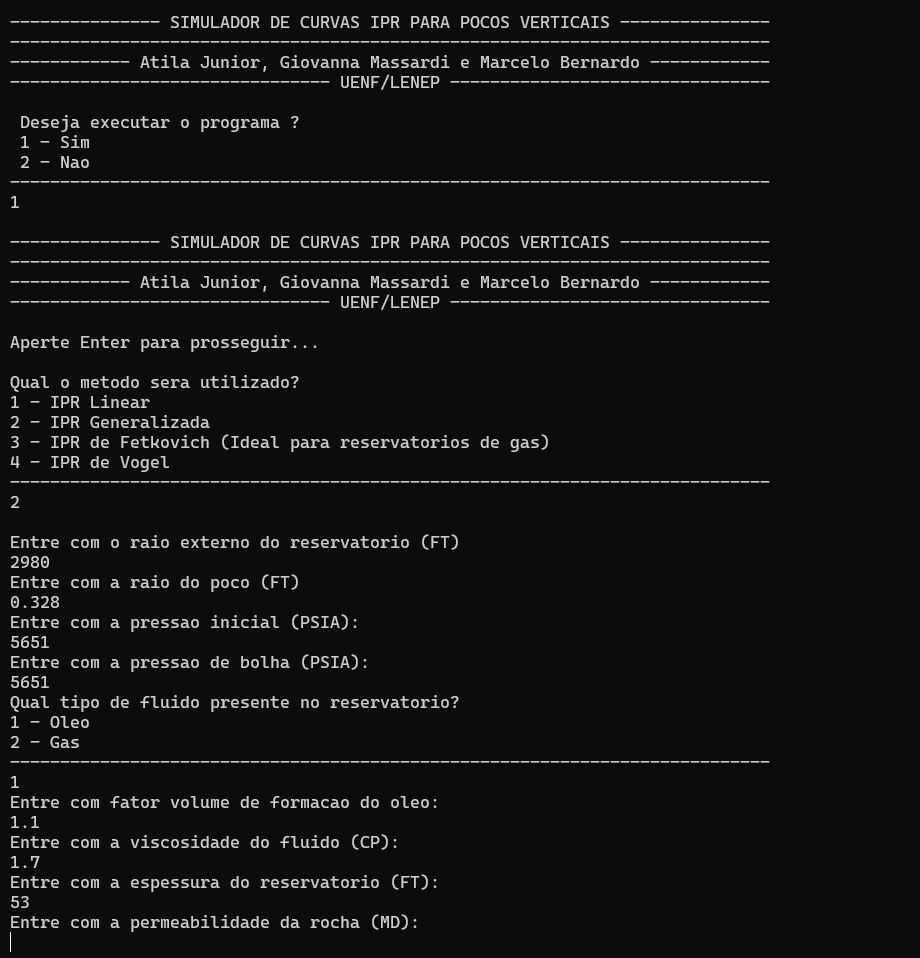
\includegraphics[width=1\textwidth]{imagens/EntradaDados}
\par\end{centering}
\caption{Software - Entrada de dados.\label{fig:Software-Entrada-Dados}}
\end{figure}

\lstset{style=out} \lstinputlisting[ caption={Exemplo teste 1}, label={CTipoFluido-h},extendedchars=true,breaklines=true,basicstyle=\footnotesize\tt] {../../test/Teste-01-Vogel.txt}


\section{Teste 2\label{sec:Teste-2}: C�lculos}

Ap�s a entrada de dados � realizado o c�lculo de vaz�es com base no
m�todo selecionado. A sa�da dos resultados � gerada com o valor de
vaz�o para a press�o de fundo em quest�o\ref{fig:Calculos}.

\begin{figure}[H]
\begin{centering}
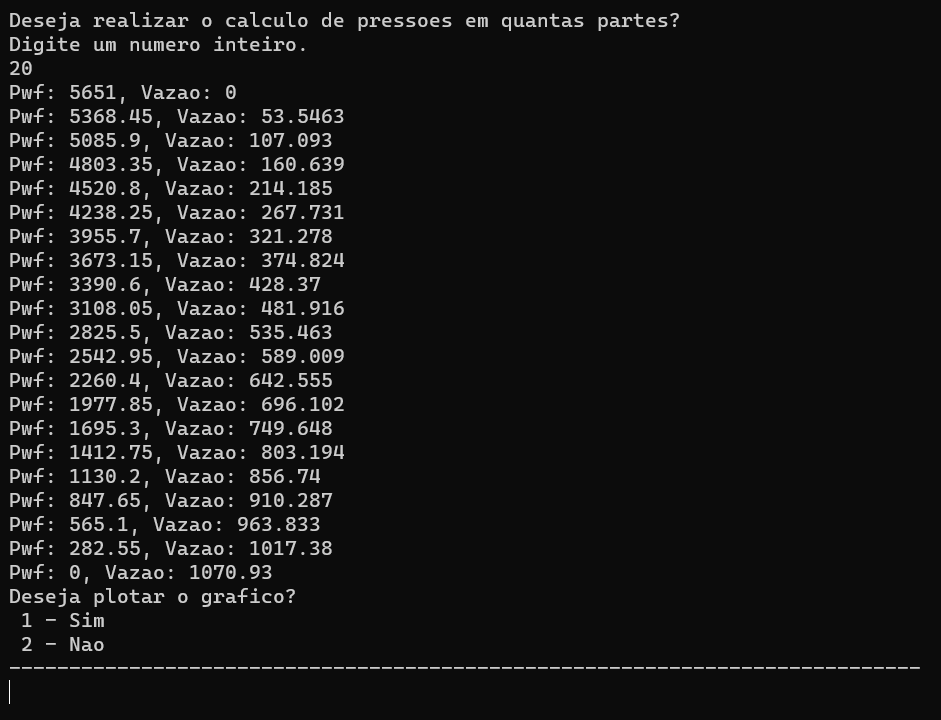
\includegraphics[width=1\textwidth]{imagens/CalculoMetodos}
\par\end{centering}
\caption{C�lculo de vaz�o.\label{fig:Calculos}}
\end{figure}


\section{Teste 3\label{sec:Teste-3}: Plotar gr�ficos}

Ap�s a entrada de dados e c�lculo dos resultados o usu�rio pode optar
pelo plot das curvas. Os resultados quando comparados � literatura
foram satisfat�rios \ref{fig:Plot-graficos}.

\begin{figure}[H]
\begin{centering}
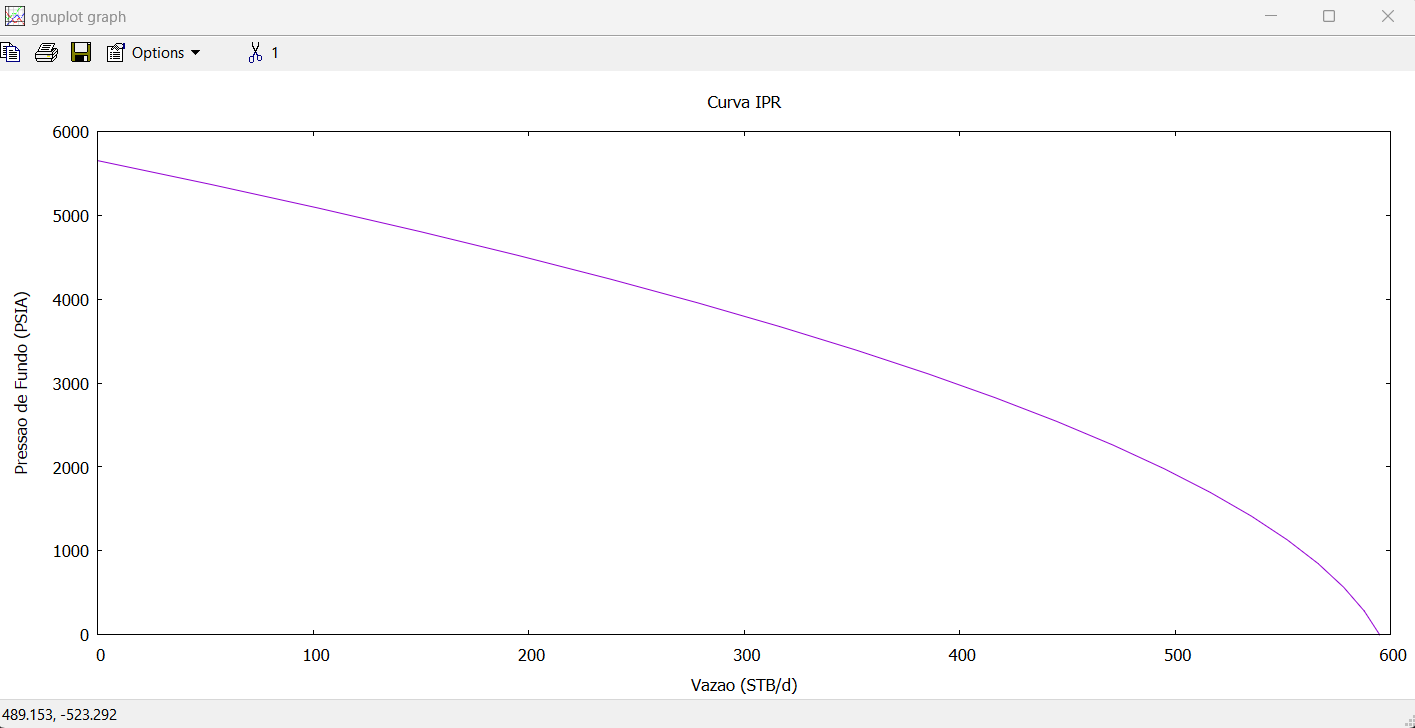
\includegraphics[width=1\textwidth]{imagens/Plotar-Graficos}
\par\end{centering}
\caption{Gr�fico IPR generalizada\label{fig:Plot-graficos}}
\end{figure}


\section{Teste 4\label{sec:Teste-4}: Salvar gr�ficos}

Ap�s o gr�fico ser gerado o usu�rio possui a autonomia de salvar o
gr�fico e executar novamente o programa para utilizar outros m�todos
de c�lculo de IPR \ref{fig:Salvar-Graficos}.

\begin{figure}[H]
\begin{centering}
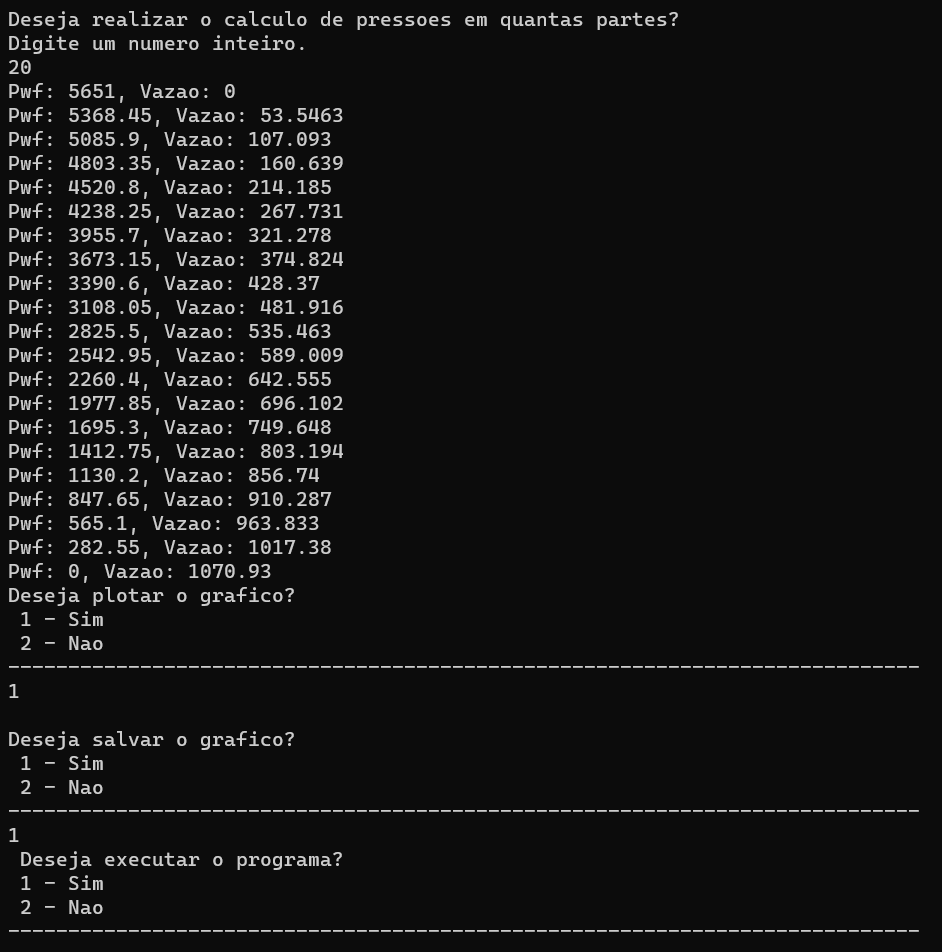
\includegraphics[width=1\textwidth]{imagens/SalvarGraficos}
\par\end{centering}
\caption{Gr�fico IPR generalizada\label{fig:Salvar-Graficos}}
\end{figure}

